% Drawing figure 1, illustration of life cycle labor supply
%\hypertarget{OptimalSupply}
\begin{figure}[tbp]
 \centerline{
  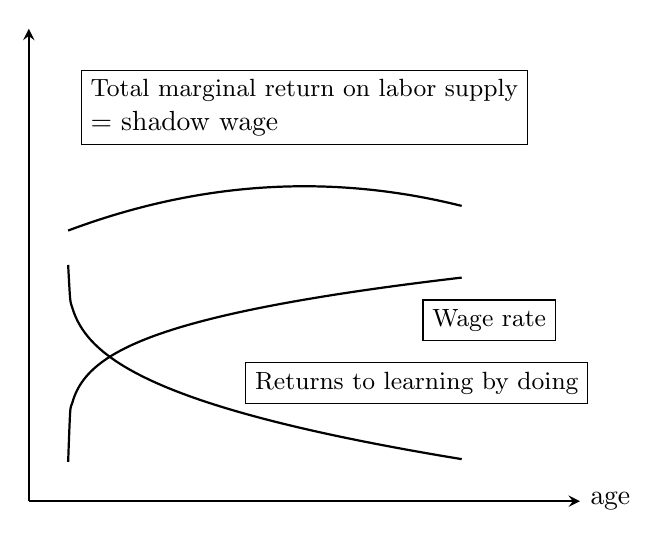
\begin{tikzpicture}
\draw[-stealth, black, thick] (0,0) -- (7,0) node[right] { age};
\draw[-stealth, black, thick] (0,0) -- (0,6);
\draw[thick, smooth, samples=200, xshift=.5cm, yshift=.5cm, domain=0:5] plot ({ \x, {(6*\x)^(1/4)}});
\node[right] at (5,2.3) [rectangle,draw] {\small Wage rate};
\draw[thick, smooth, samples=200, xshift=.5cm, yshift=3cm, domain=0:5] plot ({ \x, {-(3*\x)^(1/3)}});
\node[right] at (2.75,1.5) [rectangle,draw] {\small Returns to learning by doing};
% \draw[thick, smooth, samples=200, xshift=.5cm, yshift=2.5cm, domain=0.05:2.05] plot ({ \x, {\x^(1/2)-\x^(1/3)}});
\draw[thick, smooth, samples=200, xshift=-.5cm, yshift=2cm, domain=1:6] plot ({ \x, {2-(\x/4 - 1)^2}});
\node[align=left] at (3.5,5) [rectangle,draw] {\small Total marginal return on labor supply \\ = shadow wage};
\end{tikzpicture}
}
\caption{OPTIMAL LIFE CYCLE LABOR SUPPLY}
\label{fig:OptimalSupply}
\end{figure}